  \subsection{Principe de fonctionnement de notre solution}
	  \paragraph{}
	  	Les factures d'un utilisateur sont identifi\'ees gr\^ace \`a la r\'ef\'erence abonn\'ee fournie \`a l'inscription. Une fois connect\'e \`a l'application, le client dispose de la liste de ses factures. Il peut donc s\'electionner la ou les factures qu'il d\'esire solder et proc\'eder au paiement. Le progiciel Gd'Or g\'en\`ere tous les jours \`a une heure pr\'ecise 00H un fichier contenant les factures impay\'ees de tous les compteurs conventionnels de la SBEE. Ce fichier est reçu par le serveur d'application et est ensuite charg\'e dans la  base de donn\'ee par une t\^ache automatique \`a 00h 30min. Ainsi nous disposons des impay\'ees au niveau des compteurs. Cependant une t\^ache doit \^etre effectu\'ee au pr\'ealable. A chaque fin de journ\'ee, \`a 00H 5min, notre application g\'en\`ere un fichier contenant toutes les factures qui ont \'et\'e pay\'ees dans la journ\'ee pr\'ec\'edente c'est \`a dire avant 00H. Nous consid\'erons ce ficher comme un bilan fait par notre application \`a Gd'Or. Ce fichier permet \`a Gd'Or de valider les paiements et d'apurer les comptes en fonction des informations fournies par les prestataires de solution de paiement avant la génération des impayés du jour suivant.
	  \paragraph{}
	  	En effet, les prestataires des diff\'erentes solutions de paiements sont aussi tenus de rendre des comptes \`a Gd'Or. Etant donn\'e qu'il s'agit de finances, rien ne doit \^etre pris \`a la l\'eg\`ere. Gd'Or \'evalue minutieusement les diff\'erents fichiers re\c{c}us et g\'en\`ere des fichiers retours en cas d'erreurs.  Les erreurs notifi\'ees sont imm\'ediatement signal\'ees aux entit\'es concern\'ees et qui doivent y apporter des solutions le plus t\^ot possible. Aussi un agent v\'erifiera tous les matins si tout s'est bien pass\'e la nuit pr\'ec\'edente. Il s'agit juste d'un contr\^ole de routine. L'automatisation de ces t\^aches, nous permet d'\'eviter au maximum des erreurs ou des retards dus \`a l'interaction homme-machine. Tous les \'echanges de fichiers se feront via un canal s\'ecuris\'e \gls{sftp} (SSH File Transfer Protocol) ou VPN (Virtual Private Network).
	  \paragraph{}
	  	Les r\`egles appliqu\'ees aux diff\'erents pare-feu et serveurs nous permettent de limiter les \'echanges entre les serveurs et les autres entit\'es. Le fichier facture contenant des impay\'ees ne peut donc pas \^etre re\c{c}u depuis n'importe quelle destination. Gd'Or est la seule entit\'e capable d'effectuer cette action. Apr\`es utilisation, les fichiers sont archiv\'es et compressés de façon automatique en format \textit{.xz} afin de garder une trace des \'echanges, des flux de donn\'ees et de sauver consid\'erablement de l'espace disque.
	  	
	  		  	
		\begin{figure}[H]
		     \begin{center}
			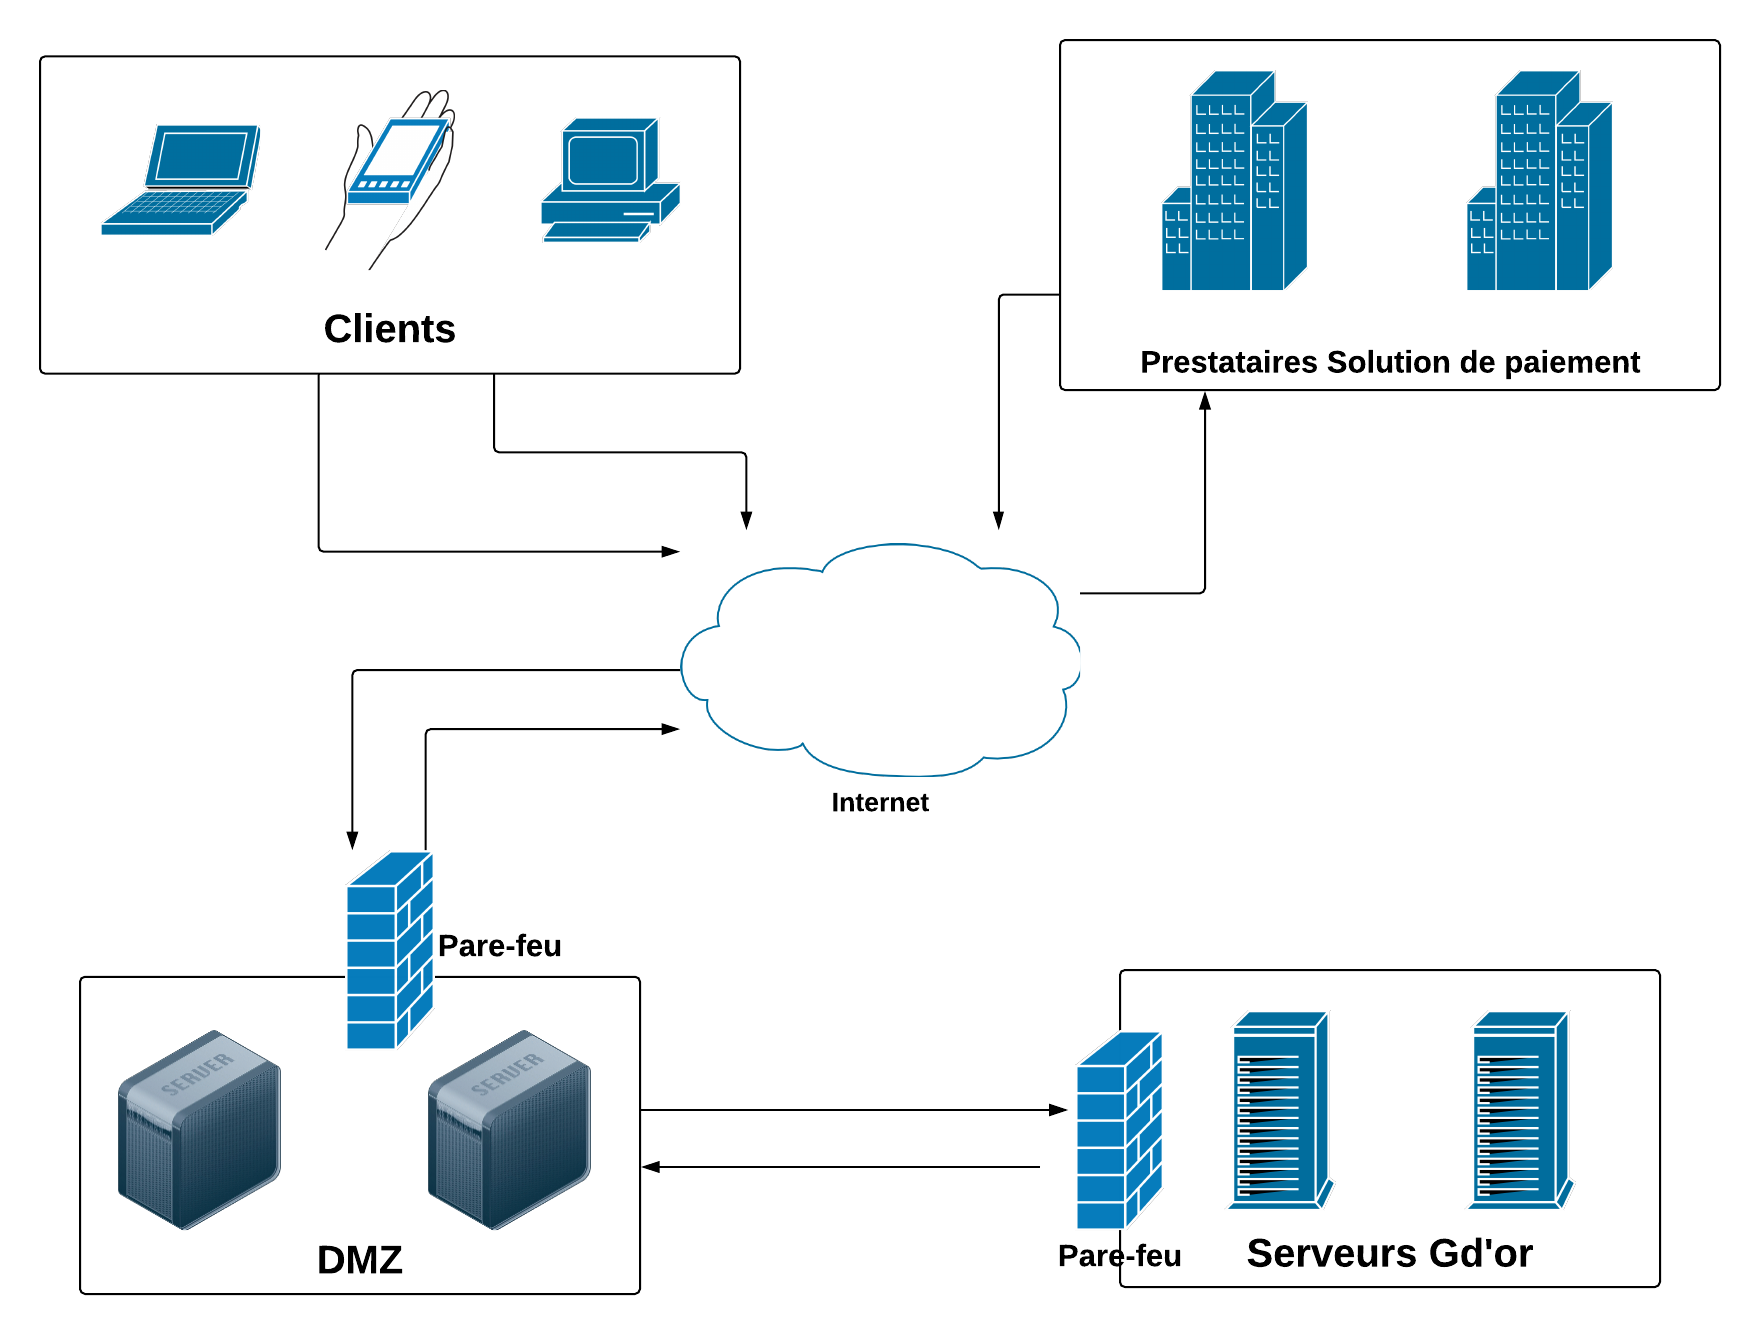
\includegraphics[scale=0.5]{images/fonctionnement.png}
		     \end{center}
		     \caption{Illustration du principe de fonctionnement}
		     \label{Diagramme de cas d'utilisation}
		\end{figure}
		
		
  \subsection{Contr\^ole des acc\`es: RBAC}
      \paragraph{}
      Il existe plusieurs façons de gérer les autorisations des utilisateurs dans un projet. Dans notre cas nous avons pens\'e \`a ce m\'ecanisme appel\'e en anglais \textbf{Role Based Access Control (RBAC)}. On pourrait juste pour faire simple  consid\'erer un rôle comme un type d'utilisateur. Ce type utilisateur n'ayant pas droit \`a toutes les fonctionnalit\'es de la plateforme, est limit\'e par des permissions ou autorisations. Conceptuellement les rôles représentent une collection nommée d'autorisations. Par exemple supposons que nous ajoutons une nouvelle fonctionnalité qui permet à un utilisateur de modifier certains paramètres importants. Cette fonctionnalité doit être disponible uniquement pour les administrateurs. Dans ce cas on associe au rôle \textbf{Administrateur} cette autorisation: \textbf{Modifier tels param\`etres}. Ainsi seuls les administrateurs ont la possibilit\'e d'effectuer cette action. L'implémentation du contrôle d'accès basé sur les rôles permet de protéger les données contre les fuites, de limiter les actions, de réduire le travail de support administratif et informatique et de répondre plus facilement aux exigences d'audit.
      
      \begin{figure}[H]
	  \begin{center}
	      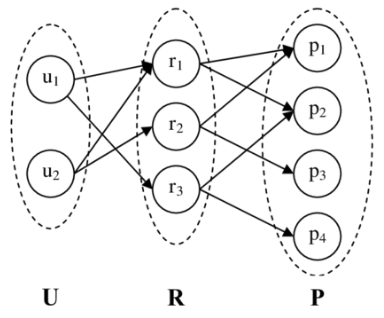
\includegraphics[scale=0.6]{images/rbac.png}
	  \end{center}
	  \caption{Repr\'esentation Utilisateurs - R\^oles - Permissions}
	  \label{Page de la whitelist IP}
      \end{figure}
      
      \paragraph{}
      Dans notre cas de figure nous disposons de trois types d'utilisateurs:
	\begin{itemize}
	
	  \item \textbf{Abonn\'e}
	    \\Les abonn\'es, ou clients, ou utilisateurs simples sont ceux qui poss\`edent un compte. Tout compte \'etant associ\'e \`a une r\'ef\'erence abonn\'e, ce type d'utilisateur dispose de plusieurs permissions. Ils sont habilit\'es \`a voir leurs propres factures, les payer, voir et modifier les informations de leur compte.
	  
	  \item \textbf{Vendeur}
	    \\Les vendeurs ont \'et\'e pens\'es afin de permettre aux personnes incapables d'utiliser le num\'erique,  de payer leurs factures via le m\^eme canal. Un particulier gr\^ace \`a son stand pourrait proc\'eder au paiement des factures. Il aurait la possibilit\'e de voir les factures d'autres personnes. Cependant une discussion par rapport \`a la confidentialit\'e d'une facture et \`a la gestion des informations contenues sur cette derni\`ere nous permet par exemple d'aller en profondeur par rapport \`a ce type d'utilisateur. Pour nos livrables ce sera donc uniquement les abonn\'es et les administrateurs responsables du bon fonctionnement de la plateforme.
	  
	  \item \textbf{Administrateur}
	    \\Les administrateurs sont responsables du bon fonctionnement de la plateforme. Ils interviennent comme un support pour les abonn\'es et ils v\'efirent si les diff\'erentes t\^aches du serveur s'ex\'ecutent normalement et avec succ\`es. Par d\'efaut, ils sont aussi des abonn\'es. Ils poss\`edent alors toutes les permissions de ces derniers en plus des leurs. Leur interface leur permet de proc\'eder \`a une gestion efficace de la plateforme et des utilisateurs. Par exemple les administrateurs sont les seuls \`a pouvoir d\'esactiver un compte.
	
	\end{itemize}
	  
  \subsection{Solutions de paiement}
      	\begin{itemize}
	  \item \textbf{Mobile Money}
	  \\MTN Mobile Money est un moyen abordable et sécurisé d’effectuer des transactions financières mobiles sans compte bancaire. Son API permet à aux utilisateurs de MTN d’acheter des biens et des services en ligne en bénéficiant de la confiance et la fiabilité associées à MTN Mobile Money. Il est actuellement disponible pour les marchands ou entreprises, qui peuvent l’intégrer sur leur site Web et application grâce à quelques lignes de code. L’interface de paiement MTN Mobile Money est rapide, facile et, surtout, complètement sécurisé. \cite{momo}
	  
	  \item \textbf{PayPal}
	  \\PayPal est un service qui vous permet de payer en ligne, d'envoyer et de recevoir de l'argent sans partager vos informations bancaires. Le compte PayPal vous permet de regrouper tous vos modes de paiement en ligne dans un seul portemonnaie numérique. Avec Paypal vous payer avec juste avec votre adresse email et votre mot de passe. C'est nettement plus facile, mais aussi plus rapide et plus sûr. Paypal est disponible dans 202 pays  donc le Bénin. \cite{paypal}
	\end{itemize}
	
  \subsection{Langages de développement et outils}

      \paragraph{}
	  Notre solution est une application web. Elle est donc accessible depuis tous les systèmes d'exploitations du moment qu'un navigateur et une connexion internet sont disponibles. Elle a \'et\'e r\'ealis\'ee gr\^ace au framework Django.

	  \subsubsection{Utilisation d'un framework}
	  Lorsque l'on réalise des sites Internet, certaines t\^aches sont toujours effectu\'ees :
	  \begin{itemize}
	    \item réalisation et codage du design ;
	    \item réalisation des modules :
	    \begin{itemize}
	      \item réalisation du modèle de données concernant le module,
	      \item réalisation des formulaires d'ajout, modification et suppression des données :
	    \end{itemize}
	    \item réalisation des pages d'affichage du contenu du site ;
	    \item réalisation d'une page d'administration pour gérer les modules ;
	    \item réalisation d'un espace utilisateur avec des droits sur l'accès aux données ;
	    \item mise en place d'un plan du site ;
	  \end{itemize}
	  \paragraph{}
	  Tout cela est relativement répétitif, et si, la première fois, ça peut paraître très amusant, on en arrive rapidement à faire des copier/coller, assez mauvaise méthode car source de nombreuses erreurs. Finalement on regroupe des morceaux de code en fonctions réutilisables. À ce moment, on se rapproche de plus en plus de la notion de framework. L'avantage d'utiliser un framework existant et surtout Open Source tel que Django, c'est que nous ne sommes pas les seuls à l'utiliser, que les bugs sont donc corrigés plus rapidement, et les améliorations sont exécutées par plusieurs personnes et de manière bien mieux réfléchie. C'est d'ailleurs tout l'intérêt d'utiliser un framework. En faire moins, pour en faire plus dans le même temps.


	  \subsubsection{Pr\'esentation de Django}
	  Il existe de nombreux framework web, dans différents langages de programmation. Pourquoi utiliser spécifiquement Django et pas un autre ? Nombreuses sont les raisons qui motivent ce choix : 
	  \begin{itemize}
	    \item la simplicité d'apprentissage;
	    \item la qualité des applications réalisées;
	    \item la rapidité de développement;
	    \item la sécurité de l'application;
	    \item la facilité de maintenance des applications sur la durée;
	    \item la performance et l'optimisation de l'application.
	  \end{itemize}
	  Outres ces avantages, on bénéficie de la clarté de Python, qui permet à plusieurs développeurs de travailler sur le même projet. Le style est imposé, donc tout le monde suit les mêmes règles, ce qui facilite les travaux en équipe et la clarté du code.
	  \begin{figure}[H]
	      \begin{center}
		  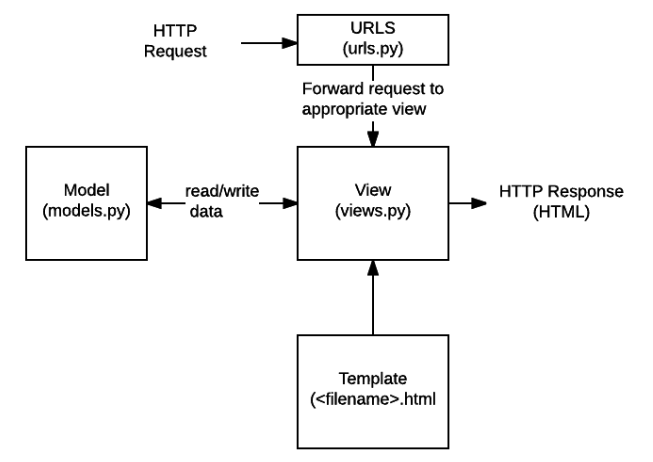
\includegraphics[scale=0.5]{images/djangoschema.png}
	      \end{center}
	      \caption{Architecture MVT Django}
	      \label{Accueil}
	  \end{figure}
	  Django se réfère à cette organisation en tant qu’architecture "Model View Template (\gls{mvt})". Il présente de nombreuses similitudes avec l’architecture plus familière de Model View Controller (\gls{mvc}).
	  
	  \subsubsection{S\'ecurit\'e avec Django}
	  La sécurité est un sujet d’importance capitale dans le développement d’applications Web et Django offre plusieurs outils et mécanismes de protection. 
	  \begin{itemize}
	    \item Protection contre le « Cross site scripting » (XSS)
	    \item Protection contre le « Cross site request forgery » (\gls{csrf})
	    \item Protection contre l’injection SQL
	    \item Protection contre le détournement de clic (« clickjacking »)
	    \item Configurations \gls{https}/\gls{ssl}
	    \item Validation de l’en-tête Host
	  \end{itemize}
	  Même si Django offre nativement de bonnes protections de sécurité, il est toujours important de déployer proprement les applications et de profiter des protections de sécurité du serveur Web, du système d’exploitation et d’autres composants. Le framework offre dans sa documentation plusieurs astuces et conseils pour am\'eliorer la s\'ecurit\'e de ses applications.

	  
  \subsubsection{Compression et Format XZ}
	XZ est un format de fichier destiné à accueillir des données compressées. C'est une spécification ouverte. Le but de ce format est d'éviter la multiplication des formats à chaque nouvel algorithme de compression. Ce format permet de choisir entre plusieurs algorithmes de compression mais aussi entre plusieurs algorithmes de vérification d'intégrité. La méthode de compression par défaut du format XZ est l'algorithme de compression LZMA2, qui est une nouvelle version de l'algorithme LZMA. Cependant XZ ne permet actuellement de choisir qu'entre ces deux algorithmes. Les algorithmes disponibles pour la vérification de l'intégrité des données compressées sont CRC-32, CRC-64 et SHA-256. Par défaut, il utilise CRC-64, qui a semblé être aux concepteurs un bon compromis entre la vitesse et la garantie d'intégrité.


	  \subsubsection{PostgreSQL}
	    PostgreSQL est un système de gestion de base de données relationnelle et objet (SGBDRO). C'est un outil libre disponible selon les termes d'une licence de type BSD. En substance, cette licence dit : « Nous mettons ce logiciel à votre disposition en l'état. Faites en ce que vous voulez. Vous pouvez le modifier ou le vendre si vous le souhaitez. Nous vous demandons juste de rappeler que nous en sommes les créateurs ».
	    Ce système est concurrent d'autres systèmes de gestion de base de données, qu'ils soient libres (comme MariaDB et Firebird), ou propriétaires (comme Oracle, MySQL, DB2 et Microsoft SQL Server). Comme les projets libres Apache et Linux, PostgreSQL n'est pas contrôlé par une seule entreprise, mais est fondé sur une communauté mondiale de développeurs et d'entreprises.
	    
	    PostgreSQL est l'une des nombreuses bases de données populaires gratuites et est fréquemment utilisée pour les bases de données Web. C'était l'un des premiers systèmes de gestion de base de données à être développé, et il permet aux utilisateurs de gérer des données structurées et non structurées. Il peut également être utilisé sur la plupart des grandes plates-formes, y compris celles basées sur Linux, et il est assez simple d'importer des informations à partir d'autres types de bases de données.

	    PostgreSQL se concentre traditionnellement sur la robustesse et la fiabilité, l'intégrité des données et les fonctionnalités destinées aux développeurs d'applications. PostgreSQL dispose d'un planificateur de requêtes sophistiqué, capable de joindre efficacement un assez grand nombre de tables. Il dispose de plusieurs avantages et son efficacit\'e n'est plus \`a d\'emontrer. 

	    \begin{itemize}
	      \item Ce moteur de gestion de base de données est évolutif et peut gérer des téraoctets de données.
	      \item Il dispose d'une implémentation solide des spécifications SQL standard
	      \item Il prend en charge les fonctionnalités SQL avancées telles que les expressions de table communes et les fonctions Windows
	      \item PL / pgSQL qui est son langage de programmation procédural interagit très bien avec SQL
	      \item Si vous êtes habitué aux mécanismes d'optimisation des performances Oracle ou MS SQL Server, PostgreSQL est votre choix
	      \item PostgreSQL a un avantage en matière de conservation et de maintien de l'intégrité des données
	    \end{itemize}
	    
	    
	  \subsubsection{Ubuntu 16.04 LTS}
	    Ubuntu est un système d’exploitation GNU/Linux basé sur la distribution Linux Debian. Ubuntu 16.04 \gls{lts} est la 6ème version LTS\footnote{Long Term Support} de ce système d'exploitation. Elle apporte plusieurs nouvelles fonctionnalités et améliorations. Compte tenu de leur cycle de support, les versions LTS conviennent mieux aux entreprises et aux utilisateurs finaux qui n'aiment pas mettre à jour leur système d'exploitation de temps en temps. Il est simple et est constitué de milliers de paquets. Les paquets sont des composants logiciels précompilés conçus pour s'installer facilement sur la machine hôte. Son aspect libre permet à plusieurs programmeurs de pouvoir identifier les failles de sécurité ou de créer plusieurs modules pour faire des tâches qui s'avèrent indispensables. Tous nos travaux ont \'et\'e r\'ealis\'es sous ce syst\`eme d'exploitation.
	    

      \subsection{Environnement de Production}
	\paragraph{}
	  L’architecture est la façon dont les composants d'une chose s’organisent. S’agissant d’un système d'information en réseau, l'objectif est d'organiser et d'exploiter ce système de manière à pouvoir le contrôler les entit\'es et à détecter des activités inattendues, indésirables et malveillantes. 
	  Actuellement, la SBEE ne dispose pas d'une DMZ au niveau de son architecture r\'es\'eau. Sur la figure suivante, nous proposons la mise en place d'une DMZ afin de mieux assurer la bon fonctionnement et la securit\'e de tout le syst\`eme apr\`es la mise en production de la solution, qui sera g\'er\'e \`a l'interne.

	  \begin{figure}[H]
	    \begin{center}
	      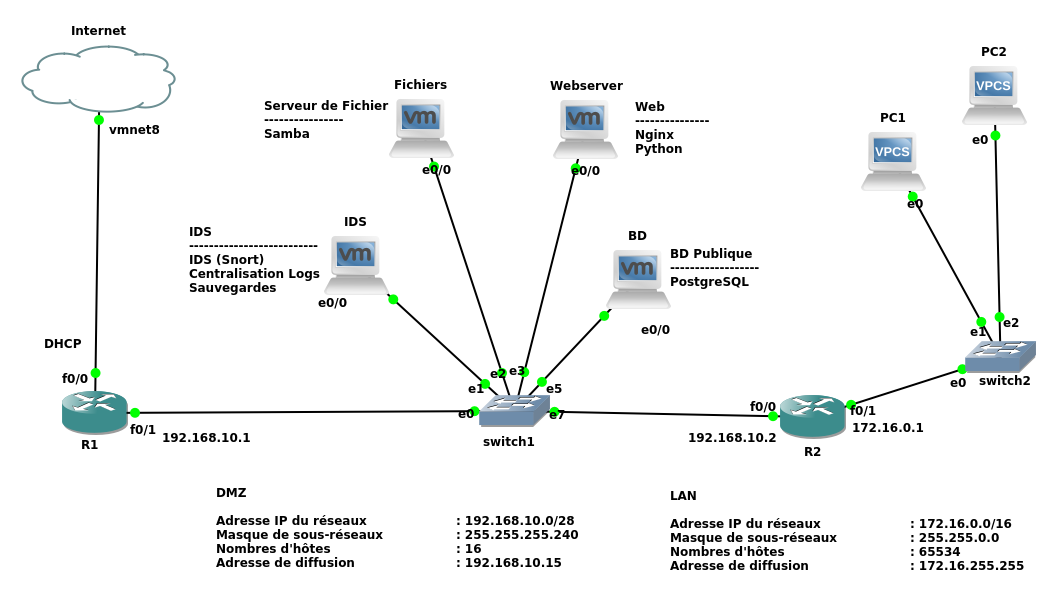
\includegraphics[scale=0.55]{images/mynetwork.png}
	    \end{center}
	    \caption[Topologie du r\'eseau]{Topologie du r\'eseau\footnotemark}
	    \label{mynetwork}
	  \end{figure}
	  \footnotetext{R\'ealis\'e par moi m\^eme avec GNS3}
	  
	  
	  \subsubsection{Serveur Web}
	    \paragraph{}
	    Le terme de serveur Web peut en général se référer à deux choses différentes : soit au \textbf{logiciel d’un serveur Web}, soit à la \textbf{machine} sur laquelle s’exécute le programme. Lorsqu’il s’agit de la seconde définition, on parle généralement d’hébergeur ou d’hôte (un tel hébergeur peut abriter plusieurs programmes de serveur Web). Dans la suite de ce guide, nous parlerons de \textbf{logiciels de serveurs Web} (ou programmes) ou d’\textbf{hébergeurs} (hôtes) pour distinguer ces deux définitions.\\
	    \begin{enumerate}
	      \item \textbf{Nginx}
		\\Chaque site Web avec un trafic croissant ou des pics de trafic importants est vulnérable aux problèmes de performances et aux temps d'arrêt, qui surviennent souvent au pire des moments, c'est-à-dire aux heures les plus chargées. En outre, presque tous les sites Web souffrent de problèmes de performances et de temps d'arrêt au fur et \`a mesure que le volume de trafic augmente régulièrement ou qu'ils subissent des pics d'utilisation importants. Nginx a été initialement développé pour résoudre le problème C10K\footnote{Probl\`eme qu'avait les autres serveurs \`a g\'erer 10 000 connexions simultanées}, c’est-à-dire pour prendre en charge facilement 10 000 connexions simultanées ou plus. L'utilisation de Nginx comme serveur Web pour notre application Python nous offre de meilleurs performances.

		\begin{figure}[H]
		    \begin{center}
			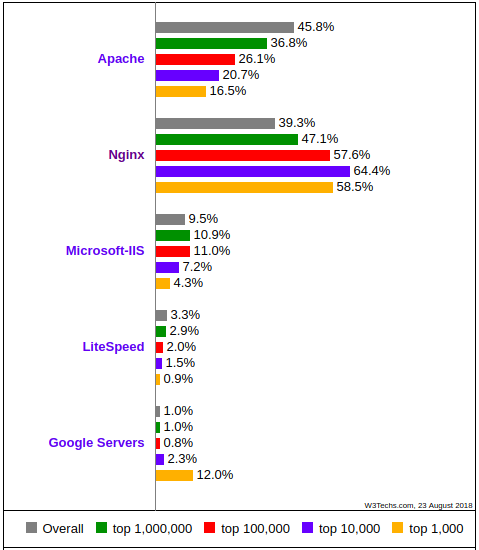
\includegraphics[scale=0.5]{images/nginx-ranking.png}
		    \end{center}
		    \caption{Pourcentages de sites Web utilisant différents serveurs Web \cite{ranking}}
		    \label{Accueil}
		\end{figure}			  
		NGNIX améliore les performances d'un site Web de trois manières différentes:
		\begin{itemize}
		  \item En tant que serveur Web
		  \item En tant que serveur proxy inverse
		  \item En tant qu'équilibreur de charge pour plusieurs serveurs d'applications
		\end{itemize}
		Plusieurs sites \`a succ\`es utilisent nginx :  Disqus, Instagram, Twitch, Wordpress, Pinterest, etc.
		%Il peut \^etre utilis\'e comme serveur Web pour notre application Python, comme serveur proxy inverse, comme équilibreur de charge ou pour les trois objectifs.
		
		\begin{figure}[H]
		    \begin{center}
			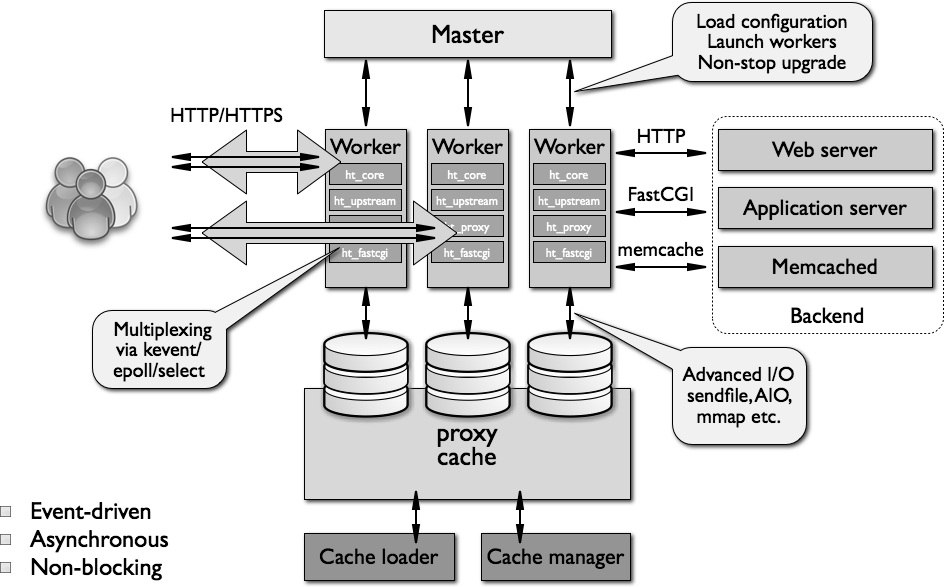
\includegraphics[scale=0.5]{images/nginxpython.png}
		    \end{center}
		    \caption{Architecture de NGINX\cite{nginx}}
		    \label{Accueil}
		\end{figure}
		Dans le sch\'ema, un serveur d’applications Python s’inscrit dans le bloc du serveur d’applications du serveur principal, et FastCGI l’a montré. NGINX ne sait pas comment exécuter Python, il a donc besoin d'une passerelle vers un environnement qui le fait. FastCGI est une interface largement utilisée pour Python, PHP et d'autres langages.
				
		
	      \item \textbf{Python}
		\\Python est un langage de programmation populaire. Il a été créé en 1991 par Guido Van Rossum.
		Il est utilisé pour:
		\begin{itemize}
		  \item le développement web (côté serveur),
		  \item le développement de logiciels,
		  \item les mathématiques et bien d'autres choses.
		\end{itemize}
		
		Django est un framework Web Python qui encourage un développement rapide et une conception propre et pragmatique. Conçu par des développeurs expérimentés, il prend en charge une grande partie des problèmes de développement Web, vous pouvez donc vous concentrer sur l'écriture de votre application sans avoir à réinventer la roue. Il gratuit et open source. Django prend la sécurité tr\`es au sérieux et aide les développeurs à éviter de nombreuses erreurs de sécurité courantes. Pour notre application, nous avons utilis\'e la version 1.11 qui est une version LTS et la version 3.6 de Python.
	    \end{enumerate}
	  
	  \subsubsection{Serveur de base de donn\'ees}
	    \paragraph{}
	      PostgreSQL est un système de gestion de base de données à usage général et relationnel. PostgreSQL est un logiciel gratuit et open source. Il nécessite des efforts minimums de maintenance grâce à sa stabilité. Par conséquent, pour des applications basées sur PostgreSQL, le coût total relatif \`a la maintenance est faible par rapport aux autres systèmes de gestion de base de données. Nous utiliserons la version 10 de PostgreSQL pour la mise en place de notre base de donn\'ee.
	  
	  \subsubsection{Serveur de Fichiers}
	    \paragraph{}
	      Un serveur de fichiers permet de partager des données à travers un réseau. Il possède généralement une grande quantité d'espace disque où sont déposés des fichiers. Les utilisateurs peuvent ensuite les récupérer au moyen d'un protocole de partage de fichier. Nous utiliserons Samba pour la mise en place de notre serveur de fichiers. Samba est un outil qui permet de partager des fichiers ou des dossiers entre différentes machines (ordinateur, tablettes, smartphones) qui peuvent tourner sous différents systèmes d'exploitation (Windows, OSX, Linux, Android)\cite{samba}. Cette compatibilité est son principal avantage mais il y en bien d'autres :
	      \begin{itemize}
		  \item Il possède la fiabilité et la stabilité de Linux
		  \item Il est très facile à mettre en œuvre
		  \item Il est sûr
		  \item Il est gratuit
	      \end{itemize}
	      
	  
	  \subsubsection{Intrusion Detection System (IDS)}
	    \paragraph{}
	      Disposer d’un \gls{ids} ou d’un \gls{ips} est essentiel dans une architecture de passerelle sécurisée. Généralement, l’IDS/IPS s’appuie sur une base de données de signatures pour détecter les intrusions potentielles ou les violations de la politique de sécurité, comme l'utilisation de protocoles non autorisés. La base de données de signatures dans un IDS est comparable à celle utilisée dans un système de détection de virus, notamment en cela qu’il ne produira aucune alerte pour une signature d’intrusion absente de sa base de données. Celle-ci doit donc être mise à jour régulièrement, tout comme avec un système de détection de logiciels malveillants.
		\begin{itemize}
		  \item \textbf{Snort}\\
		  Snort est capable d'effectuer en temps réel des analyses de trafic et de logger les paquets sur un réseau IP. Pour effectuer ces analyses, Snort se fonde sur des règles \cite{d}. Il est fourni avec certaines règles de base mais cependant, comme tout logiciel, Snort n'est pas infaillible et demande donc une mise à jour régulière. Snort peut également être utilisé avec d'autres projets open sources tels que SnortSnarf, \gls{acid}, sguil et BASE afin de fournir une représentation visuelle des données concernant les éventuelles intrusions. Il est l'un des plus actifs \gls{nids} Open Source et possède une communauté importante contribuant à son succès. Snort sera install\'e et configur\'e sur une machine \`a l'entr\'ee de la DMZ avant le switch. Nous pourrons détecter les attaques qui n'ont pas été filtrées par le pare-feu et qui relèvent d'un certain niveau de compétence. Aussi les logs seront ici plus clairs à consulter puisque les attaques bénignes\footnote{Trop faciles} ne seront pas recensées.

		  \item \textbf{Fail2ban}\\
		  Fail2ban est un \gls{hids} qui bloque les adresses IP appartenant à des hôtes qui tentent de casser la sécurité du système. Il lit les logs de divers services (SSH, Apache, \gls{ftp}) à la recherche d'erreurs d'authentification répétées et ajoute une règle iptables pour bannir l'adresse IP de la source \cite{i}. Il est capable de réduire le taux de tentatives d'authentification incorrectes, mais il ne peut pas éliminer le risque que présente une authentification faible.  La grande force de Fail2Ban est sa grande modularité que cela soit au niveau des mécanismes de détections basées sur les expressions régulières ou sur les actions à mener qui peuvent aller de l'expédition d'un mail à la mise en place de règles de Firewall. Fail2ban sera install\'e et configur\'e sur tous les serveurs de notre architecture.
		\end{itemize}
		
	   \subsubsection{Centralisation des journaux d’événements (logs)}
	    \paragraph{}
	      Les logs sont des éléments indispensables à toutes les applications pour comprendre le fonctionnement, analyser, diagnostiquer et intervenir en conséquence. Le dossier “/var/log” stocke l’ensemble des logs systèmes et applicatifs sous Linux via rSysLog. La centralisation des journaux d’événements permet d'avoir une vue d’ensemble d’éléments cruciaux à la bonne gestion d’un SI pour y mener des traitements. En cas de crash ou de suppression des logs sur une entit\'e, elle permet de diagnostiquer un crash et de garantir la survie des logs à une suppression. La centralisation des logs, lorsqu’elle est couplée à des outils d’analyse, de traitements, d’indexation et encore mieux, de graphage, permet d’avoir de toutes ces lignes d’information un ensemble cohérent de données qu’il est possible de corréler. Notre choix s'est donc port\'e sur Elastic Stack (ELK). Il est compos\'e de trois outils dont Elasticsearch (indexation et recherche de données), LogStash (r\'ecolte et traitement des logs) et Kibana (visualisation de donnée sous formes de graphiques).
	    

	  \subsubsection{Les r\`egles Iptables}	  
	      Un pare-feu (appelé aussi coupe-feu, garde-barrière ou firewall en anglais), est un système permettant de protéger un ordinateur ou un réseau d'ordinateurs des intrusions provenant d'un réseau tiers en filtrant les flux de donn\'ees. Lorsqu’un paquet IP rencontre une chaîne de règles dans son cheminement à travers le kernel, celui-ci vérifie si certaines r\`egles sont respect\'ees:
	      \begin{itemize}
		  \item Dès qu’une règle s’applique à un paquet, l’action prévue dans la règle est effectuée : transmettre le paquet, le supprimer ou le renvoyer au destinataire.
		  \item Lorsqu’aucune des règles ne peut s’appliquer pour le paquet, c’est la politique par défaut qui entre en vigueur. Là encore, on peut se retrouver avec les trois cas de figure : transmettre, supprimer, rejeter.
	      \end{itemize}
	  La configuration d’un pare-feu consiste donc à définir la politique par défaut ainsi qu’une série de règles pour chacune des chaînes de filtres essentielles\cite{iptables}.
	  Iptables est une solution complète et fiable de pare-feu et il dispose de très nombreuses options qui permettent de faire du filtrage très fin. Précisons dès maintenant que le module qui fournit au noyau Linux les fonctions de pare-feu, de partage de connexions internet (\gls{nat}) et d'historisation du trafic réseau s'appelle Netfilter. iptables est en fait juste l'outil qui permet à un administrateur de configurer Netfilter en mode utilisateur. Pour notre architecture, nous bloquons d'abord tout le trafic entrant par défaut. Ensuite nous autorisons au cas par cas: le trafic appartenant ou lié à des connexions déjà établies et le trafic à destination des serveurs (web, ssh, etc.) que nous mettons à disposition.
	  
	  
	  \subsubsection{Ubuntu Server 18.04 LTS}
	    Ubuntu 18.04 LTS est la derni\`ere version LTS mise en ligne le 26 Avril 2018. Elle apporte plusieurs nouvelles fonctionnalités et améliorations dont l'installeur du syst\`eme d'exploitation (Subiquity Installer). Ubuntu serveur ne dispose pas par d\'efaut d'une interface graphique. Tous les serveurs entrant en jeu dans notre travail tournent sous ce syst\`eme d'exploitation.

	  
  \section*{Conclusion}
      \paragraph{}
	  Dans ce chapitre, nous avons présenté les diff\'erents choix opérés ainsi que notre solution à travers sa modélisation, son principe de fonctionnement et les outils utilisés.
	  Le solution propos\'ee a \'et\'e r\'ealis\'ee gr\`ace au framework Django, tr\`es robuste et performant. Ensuite pour l'organisation et la structuration des differentes donn\'ees, nous utilisons PostgreSQL, qui est un système de gestion de base de données relationnelle complet, stable, performant, riche de nombreuses années de développement, en évolution constante et soutenu par une communauté active. 
	  Enfin vu que l'architecture existante \`a la SBEE ne contient pas de DMZ nous en avons propos\'ee une autre qui comble ce manque et qui nous donne un apercu de l'environnement de production puisque le tout sera g\'er\'e \`a l'interne.
	  Le chapitre suivant exposera les différents résultats et quelques critiques.
	  